\documentclass{ximera}

\author{Anna Davis} \title{MTH 160 Homework 10} 

\begin{document}

\begin{abstract}

\end{abstract}
\maketitle
 \textit{Certificate due: 4/14/2021 at 11:59 p.m.}
 \section{Lecture 23}
\begin{problem}\label{prob:160hom10prob1}
Covert each angle measure, as indicated.  Enter exact values.  Type pi to get $\pi$.
\begin{enumerate}
    \item $\frac{4\pi}{5}$ radians $=\answer{144}$ degrees.
    \item $36$ degrees $=\answer{\frac{\pi}{5}}$ radians.
    \item $\frac{5\pi}{12}$ radians $=\answer{75}$ degrees.
    \item $280$ degrees $=\answer{\frac{14\pi}{9}}$ radians.
\end{enumerate}
\end{problem}

\section{Lecture 24}

\begin{problem}\label{prob:160hom10prob2}
For angle $A$ in the triangle shown below, list the exact values of the six trigonometric functions. (Leave square roots in your expressions - do not plug into the calculator.)
\begin{image}
   
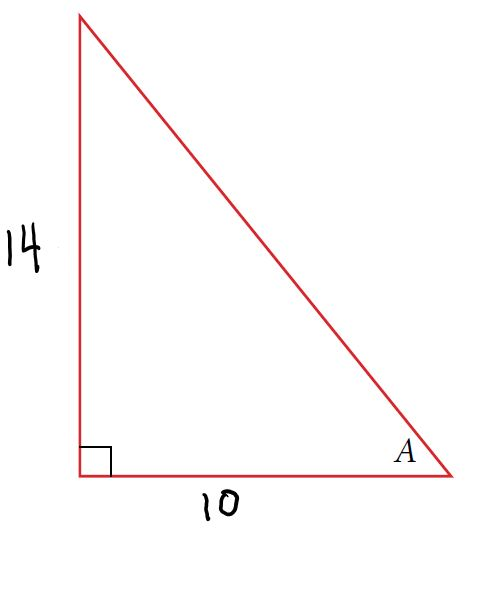
\includegraphics[height=1in]{160H10pic5.jpg}~
 
\end{image}

$$\sin A=\frac{\answer{14}}{\answer{\sqrt{296}}}\quad \csc A=\frac{\answer{\sqrt{296}}}{\answer{14}}$$

$$\cos A=\frac{\answer{10}}{\answer{\sqrt{296}}}\quad \sec A=\frac{\answer{\sqrt{296}}}{\answer{10}}$$

$$\tan A=\answer{7/5}\quad \cot A=\answer{5/7}$$
\end{problem}

\begin{problem}\label{prob:160hom10prob3}
Find the EXACT values of the six trigonometric functions for angle $\theta$. 
 
 \begin{image}
   
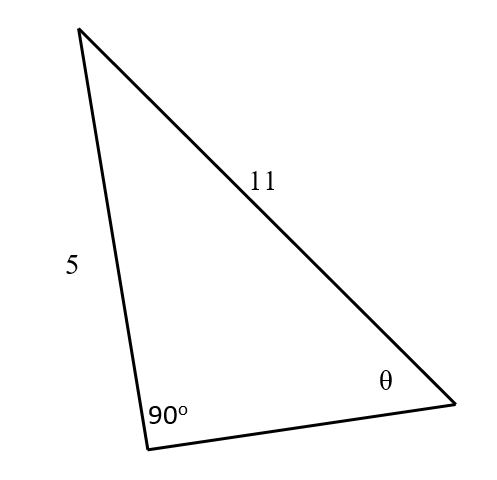
\includegraphics[height=1in]{160H10pic6.jpg}

\end{image}

$$\sin\theta=\answer{5/11},\quad \cos\theta=\answer{\frac{\sqrt{96}}{11}},\quad\tan\theta=\answer{\frac{5}{\sqrt{96}}}$$
$$\csc\theta=\answer{\frac{11}{5}},\quad\sec\theta=\answer{\frac{11}{\sqrt{96}}},\quad\cot\theta=\answer{\frac{\sqrt{96}}{5}}$$
\end{problem}

\begin{problem}\label{prob:160hom10prob4}
Find $x$.  Round your answer to one decimal place.
 
 \begin{image}
   
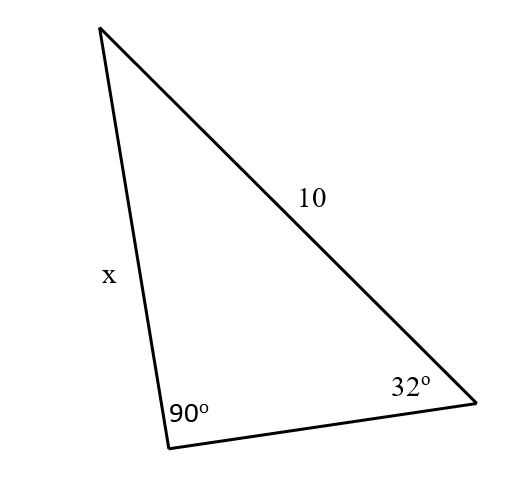
\includegraphics[height=1in]{160H10pic7.jpg}

\end{image}
$$x=\answer[tolerance=0.01]{5.3}$$
\end{problem}


\begin{problem}\label{prob:160hom10prob5}
Solve the triangle.  Enter EXACT answers (using square roots, if necessary).
\begin{image}
   
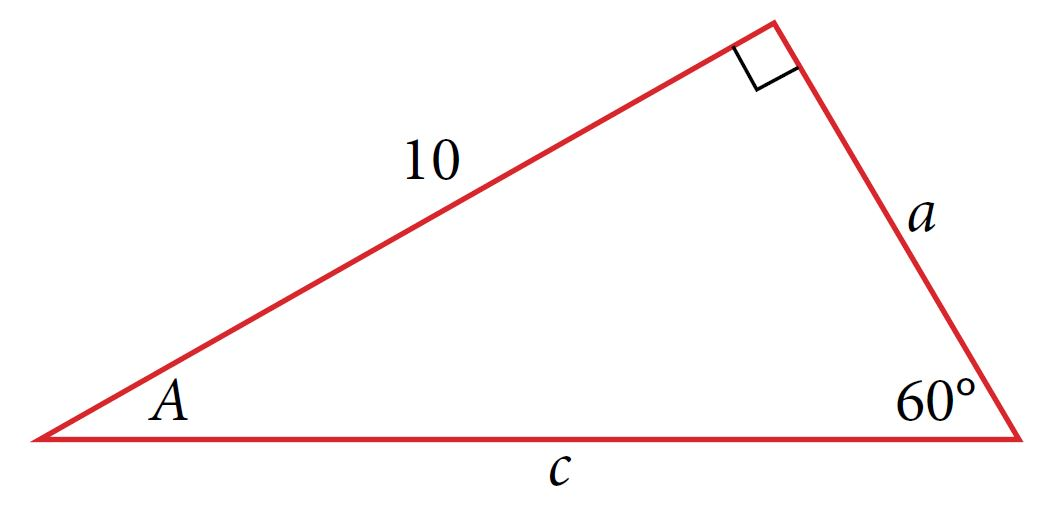
\includegraphics[height=1in]{160H10pic3.jpg}~
 
\end{image}

$$\angle A=\answer{30}\mbox{ degrees}$$
$$a=\answer{\frac{10}{\sqrt{3}}},\quad c=\answer{\frac{20}{\sqrt{3}}}$$
\end{problem}


\begin{problem}\label{prob:160hom10prob6}
Solve the triangle. Round your answers to two decimal places.
\begin{image}
   
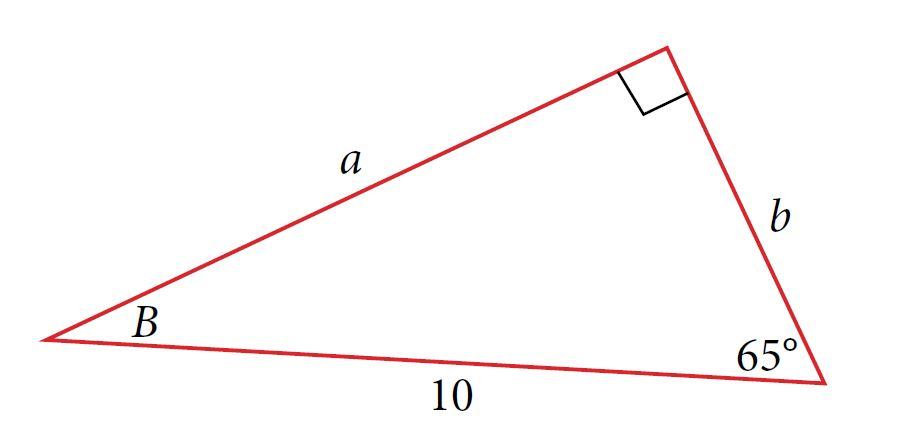
\includegraphics[height=1in]{160H10pic4.jpg}~
 
\end{image}

$$\angle B=\answer{25}\mbox{ degrees}$$
$$a=\answer[tolerance=0.001]{9.06},\quad b=\answer[tolerance=0.001]{4.23}$$
\end{problem}

\section{Lecture 25}

\begin{problem}\label{prob:160hom10prob7}
Find the missing coordinate.  Round your answers to two decimal places.
\begin{image}
   
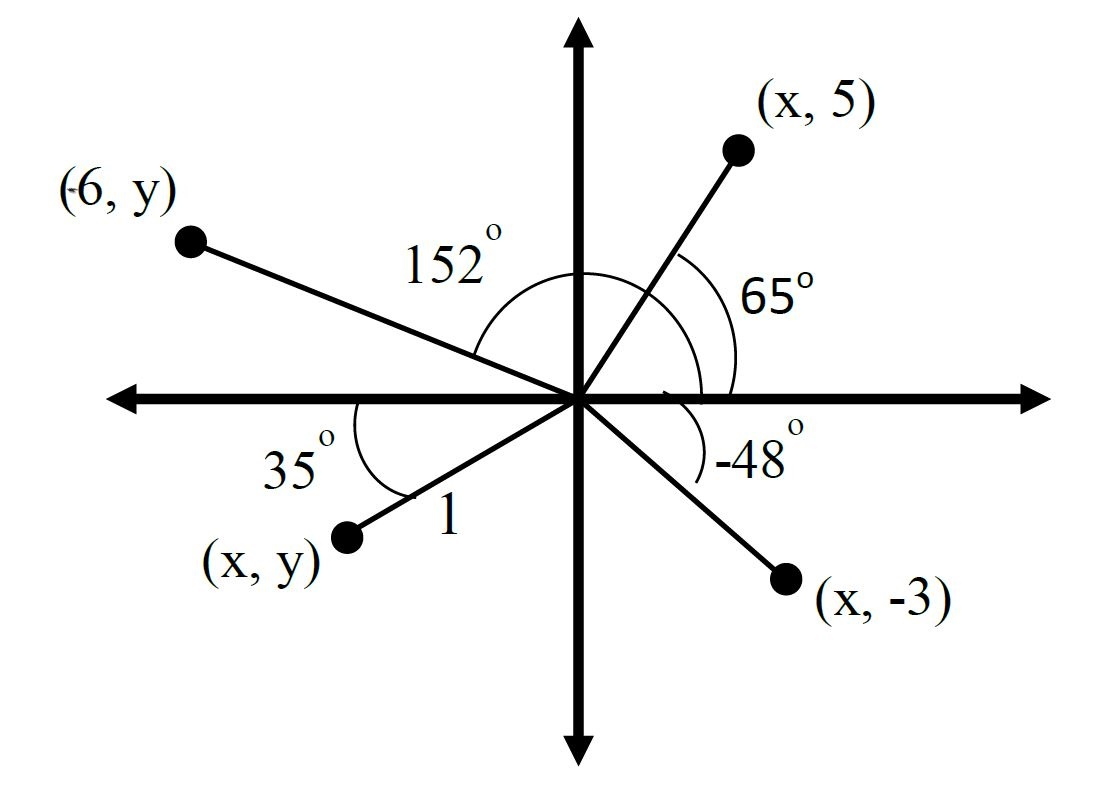
\includegraphics[height=1in]{160H10pic2.jpg}~
 
\end{image}

Quadrant I:
$$x=\answer[tolerance=0.01]{2.33}$$

Quadrant II:
$$y=\answer[tolerance=0.01]{3.19}$$

Quadrant III:
$$x=\answer{-0.82},\quad y=\answer{-0.57}$$

Quadrant IV:
$$x=\answer[tolerance=0.01]{2.7}$$
\end{problem}

\begin{problem}\label{prob:160hom10prob8}
Find $y$.  Round your answer to two decimal places.
 
 \begin{image}
   
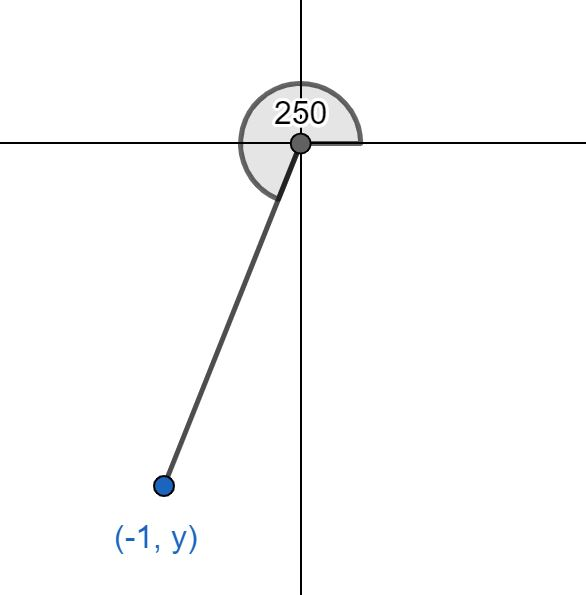
\includegraphics[height=1in]{160H10pic1.jpg}

\end{image}
$$y=\answer[tolerance=0.01]{-2.75}$$
\end{problem}


\end{document} 